\section{Поверхность потенциальной энергии межмолекулярного взаимодействия}

\begin{figure}[!ht]
	\hspace*{-1.2cm}
	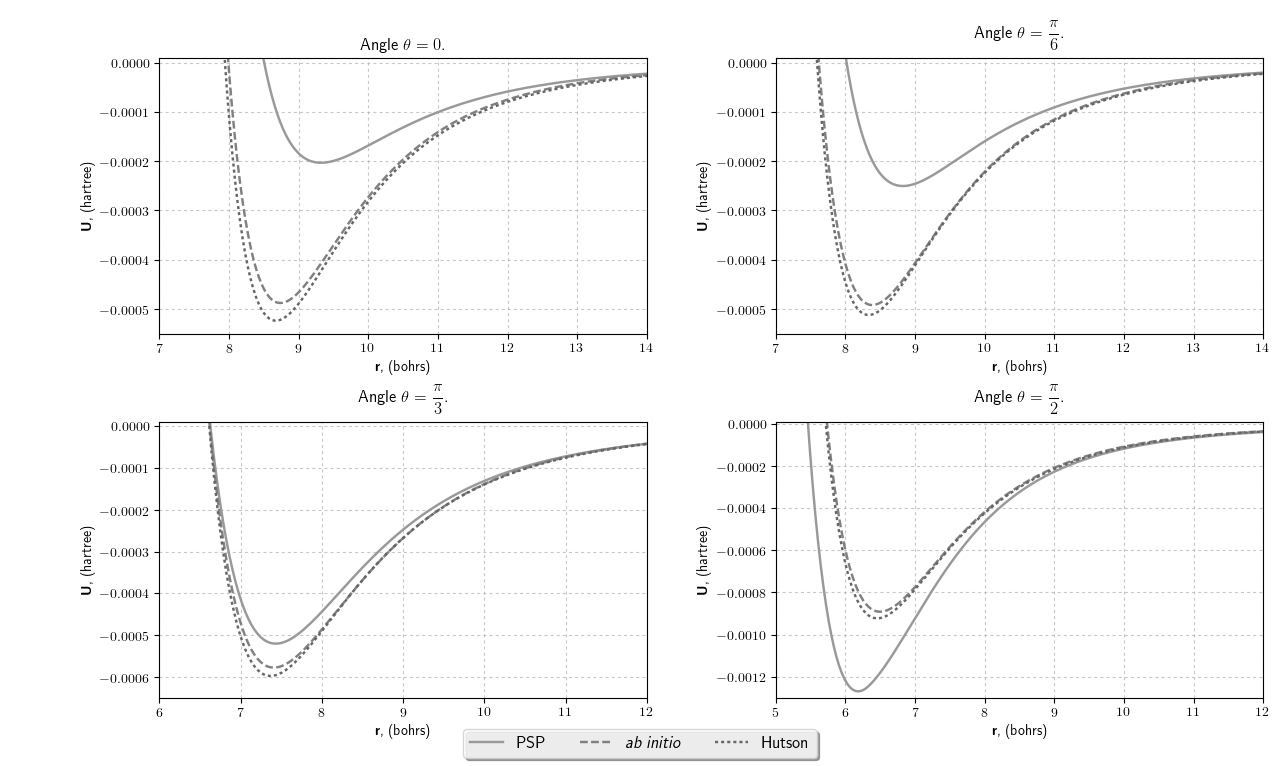
\includegraphics[width=1.1\textwidth]{pictures/potential_well.png}
	\caption{Сечения поверхностей потенциальной энергии при разных углах $\theta$ в области потенциальной ямы.}
	\label{fig:pic1}
\end{figure}

\begin{figure}[!ht]
	\hspace*{-1.2cm}
	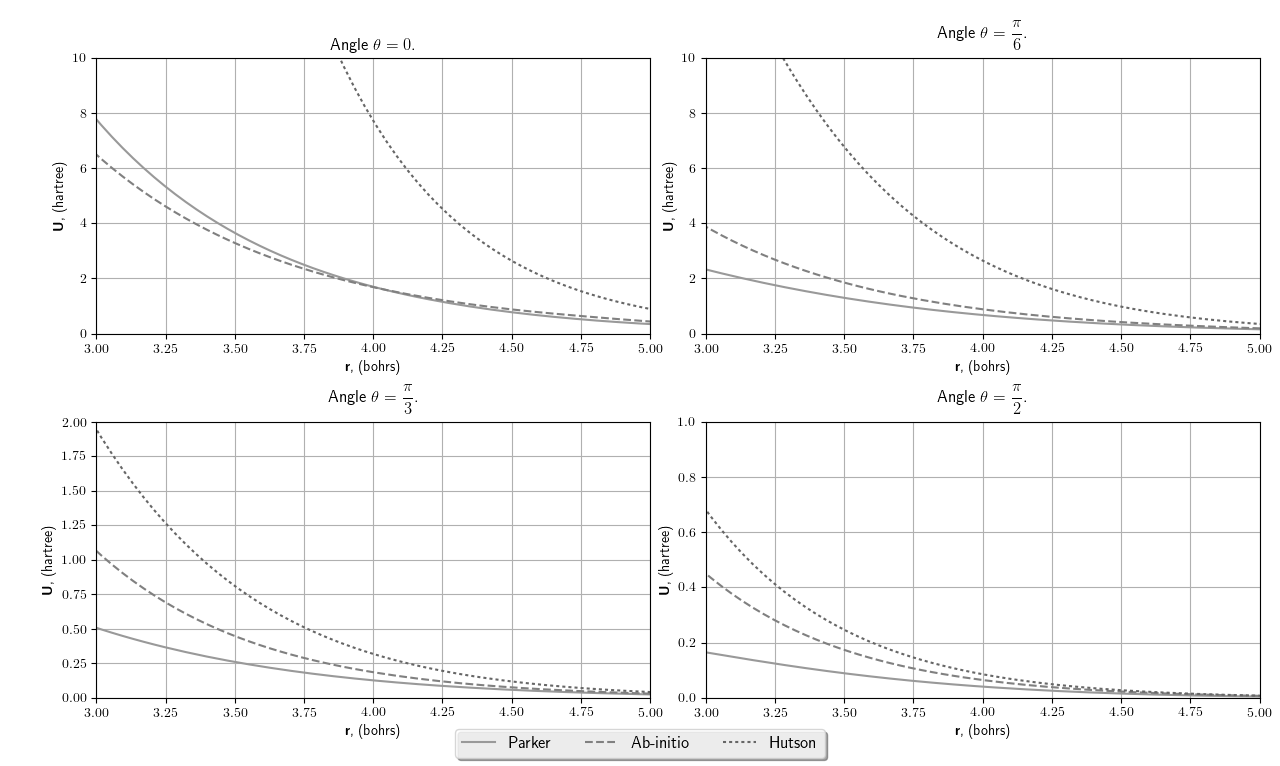
\includegraphics[width=1.1\textwidth]{pictures/potential_wall.png}
	\caption{Сечения поверхностей потенциальной энергии при разных углах $\theta$ в отталкивательной области.}
	\label{fig:pic2}
\end{figure}

Первая поверхность потенциальной энергии (обозначаемая далее P.-Parker) для системы $Ar-CO_2$ была предложена в работе \cite{parker1976}. Потенциал P. имеет потенциальную яму, которая резко выражена для Т-образной геометрии. Аналитическая форма потенциала реализована в виде разложения по полиномам Лежандра:
\vverh
\begin{gather}
	U(r, \theta) = \sum_{n = 0, 2 \dots} v_n(r) P_n \lb \cos \theta \rb, \notag
\end{gather}
в котором появляются только четные $n$ из-за $D_{\infty h}$ симметрии молекулы $CO_2$. Функции $v_n(r)$ при малых расстояниях представляют собой экспоненциальные функции (описывают резкое возрастание потенциальной поверхности), при больших расстояниях -- полиномиальные функции (описывающие Ван-дер-Ваальсово притяжение). 
\vverh
\begin{gather}
	v_n^{HF} = A_{n1} \exp \lb A_{n2} r + A_{n3} r^2 \rb, \notag \quad \quad 
	v_n^{COR} = \left\{
	\begin{aligned}
		- B_{n1}^{\, \prime} \exp \lb B_{n2} + B_{n3} r^2 \rb, \quad r \leqslant r_n \\
		-C_6(n) r^{-6} - C_8(n) r^{-8}, \quad r \geqslant r_n
	\end{aligned} \right. \notag \\
	v_n(r) = v_n^{HF} + v_n^{COR} \notag 
\end{gather}

Вторая поверхность потенциальной энергии была взята из работы \cite{hutson1996} (H. - Hutson). Т.к. эта работа была выполнена практически спустя 20 лет после первой, экспериментальные данные, на которые опирались авторы при построении потенциальной поверхности, в значительной степени пополнились. Построенная ППЭ опирается на спектроскопические данные высокого разрешения и на температурную зависимость вириального коэффициента. Аналитическое форма потенциала Лежандра.  

Наконец, третья поверхность была получена Калугиной Ю. в рамках \textit{ab-initio} расчета методом CCSD(T) в базисе \textit{aug-cc-pvqz}.

Профили потенциальной энергии при $T$-образной геометрии комплекса (соответствуют $\theta = \frac{\pi}{2}$) показывают, что потенциал P. имеет существенно большую яму чем другие два потенциала (Рис. \ref{fig:pic1}). При уменьшении угла $\theta$ видно, что разница между потенциалами H. и \textit{ab-initio} также остается небольшой, в то время как потенциальная яма P. резко изменяет свою величину с уменьшением угла $\theta$ (понятно, что потенциалы симметричны относительно плоскости, соответствующей углу $\theta = \frac{\pi}{2}$). Однако интегральная величина потенциальной ямы (усредненная по угловой координате) оказывается близка для потенциалов H. и P. \cite{hutson1996}. \par
В отталкивательной области значения потенциалов отличаются достаточно существенно (Рис. \ref{fig:pic2}).

